\chapter{Ontwerp}
In dit hoofdstuk wordt er gekeken naar het softwareontwerp, er wordt gefocust om een robuust en generiek applicatie en communicatie ontwikkelen. De applicatie is op het moment opgebouwd in verschillende onderdelen, deze onderdelen zijn de applicatie, preprocessor, sensor drivers en abstractie en communicatie.

\section{Structuur}
Voor dat er gekeken kan worden naar het ontwerp moet er een overzicht gemaakt worden hoe de applicatie uiteindelijk zich moet gaan gedragen. Hoe moet er gecommuniceerd worden, hoe kiest de applicatie welke sensor hij aan het uitlezen is dit. De volgende afbeelding geeft \ref{fig:appstructuur} geeft dit overzicht. 
\begin{figure}[h!]
	\centering
	\label{fig:appstructuur}

	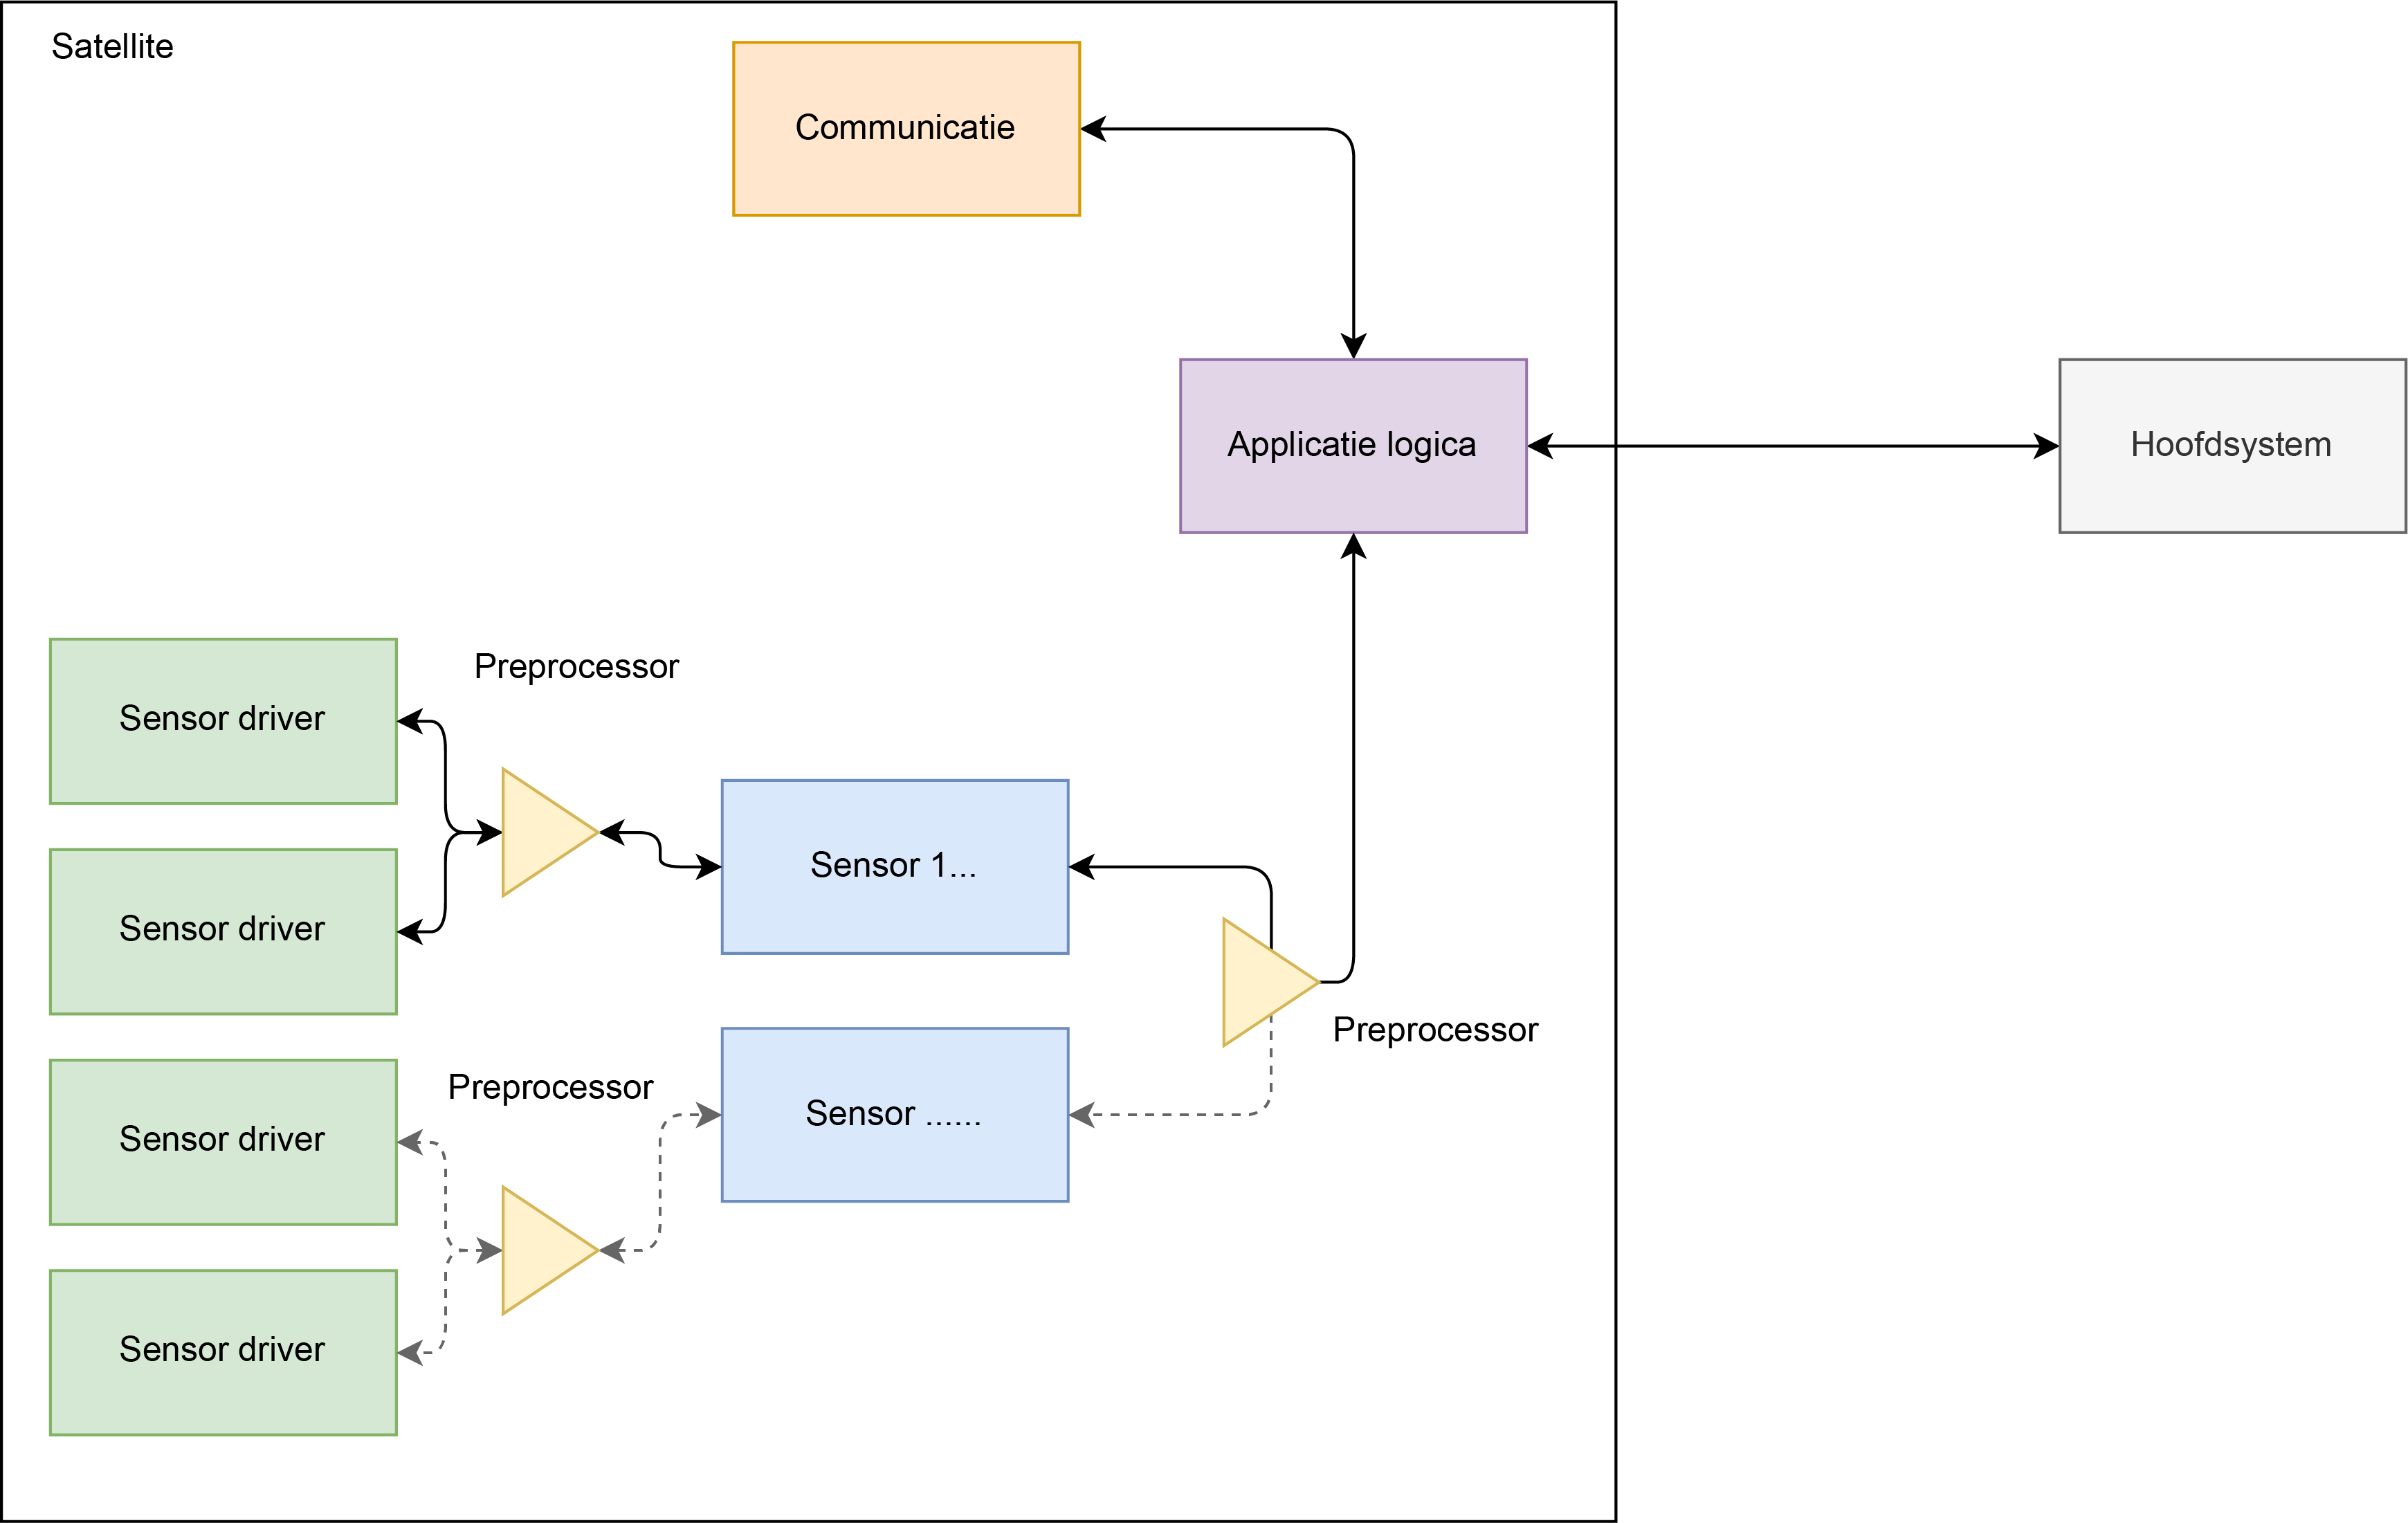
\includegraphics[width=1\linewidth]{ontwerp/compleet structuur.png}
	\caption{Algemene structuur van de applicatie}
\end{figure}

\newpage
\section{Applicatie}
De applicatie moet zo generiek mogelijk zijn, dit betekent dat de applicatie moet werken als er bijvoorbeeld van sensor verandert of toegevoegd wordt. Als er nieuwe sensor toegevoegd wordt is er een doel, het doel is dat de enige toevoeging wat er gemaakt moet worden is dat er een driver geschreven wordt voor dat specifieke sensor, maar aanpassing aan de applicatie moet minimaal gebeuren. In afbeelding \ref{fig:appontwerp} wordt een algemeen overzicht gemaakt hoe de applicatie in lagen is opgebouwd. 
\begin{figure}[h!]
	\centering
	\label{fig:appontwerp}

	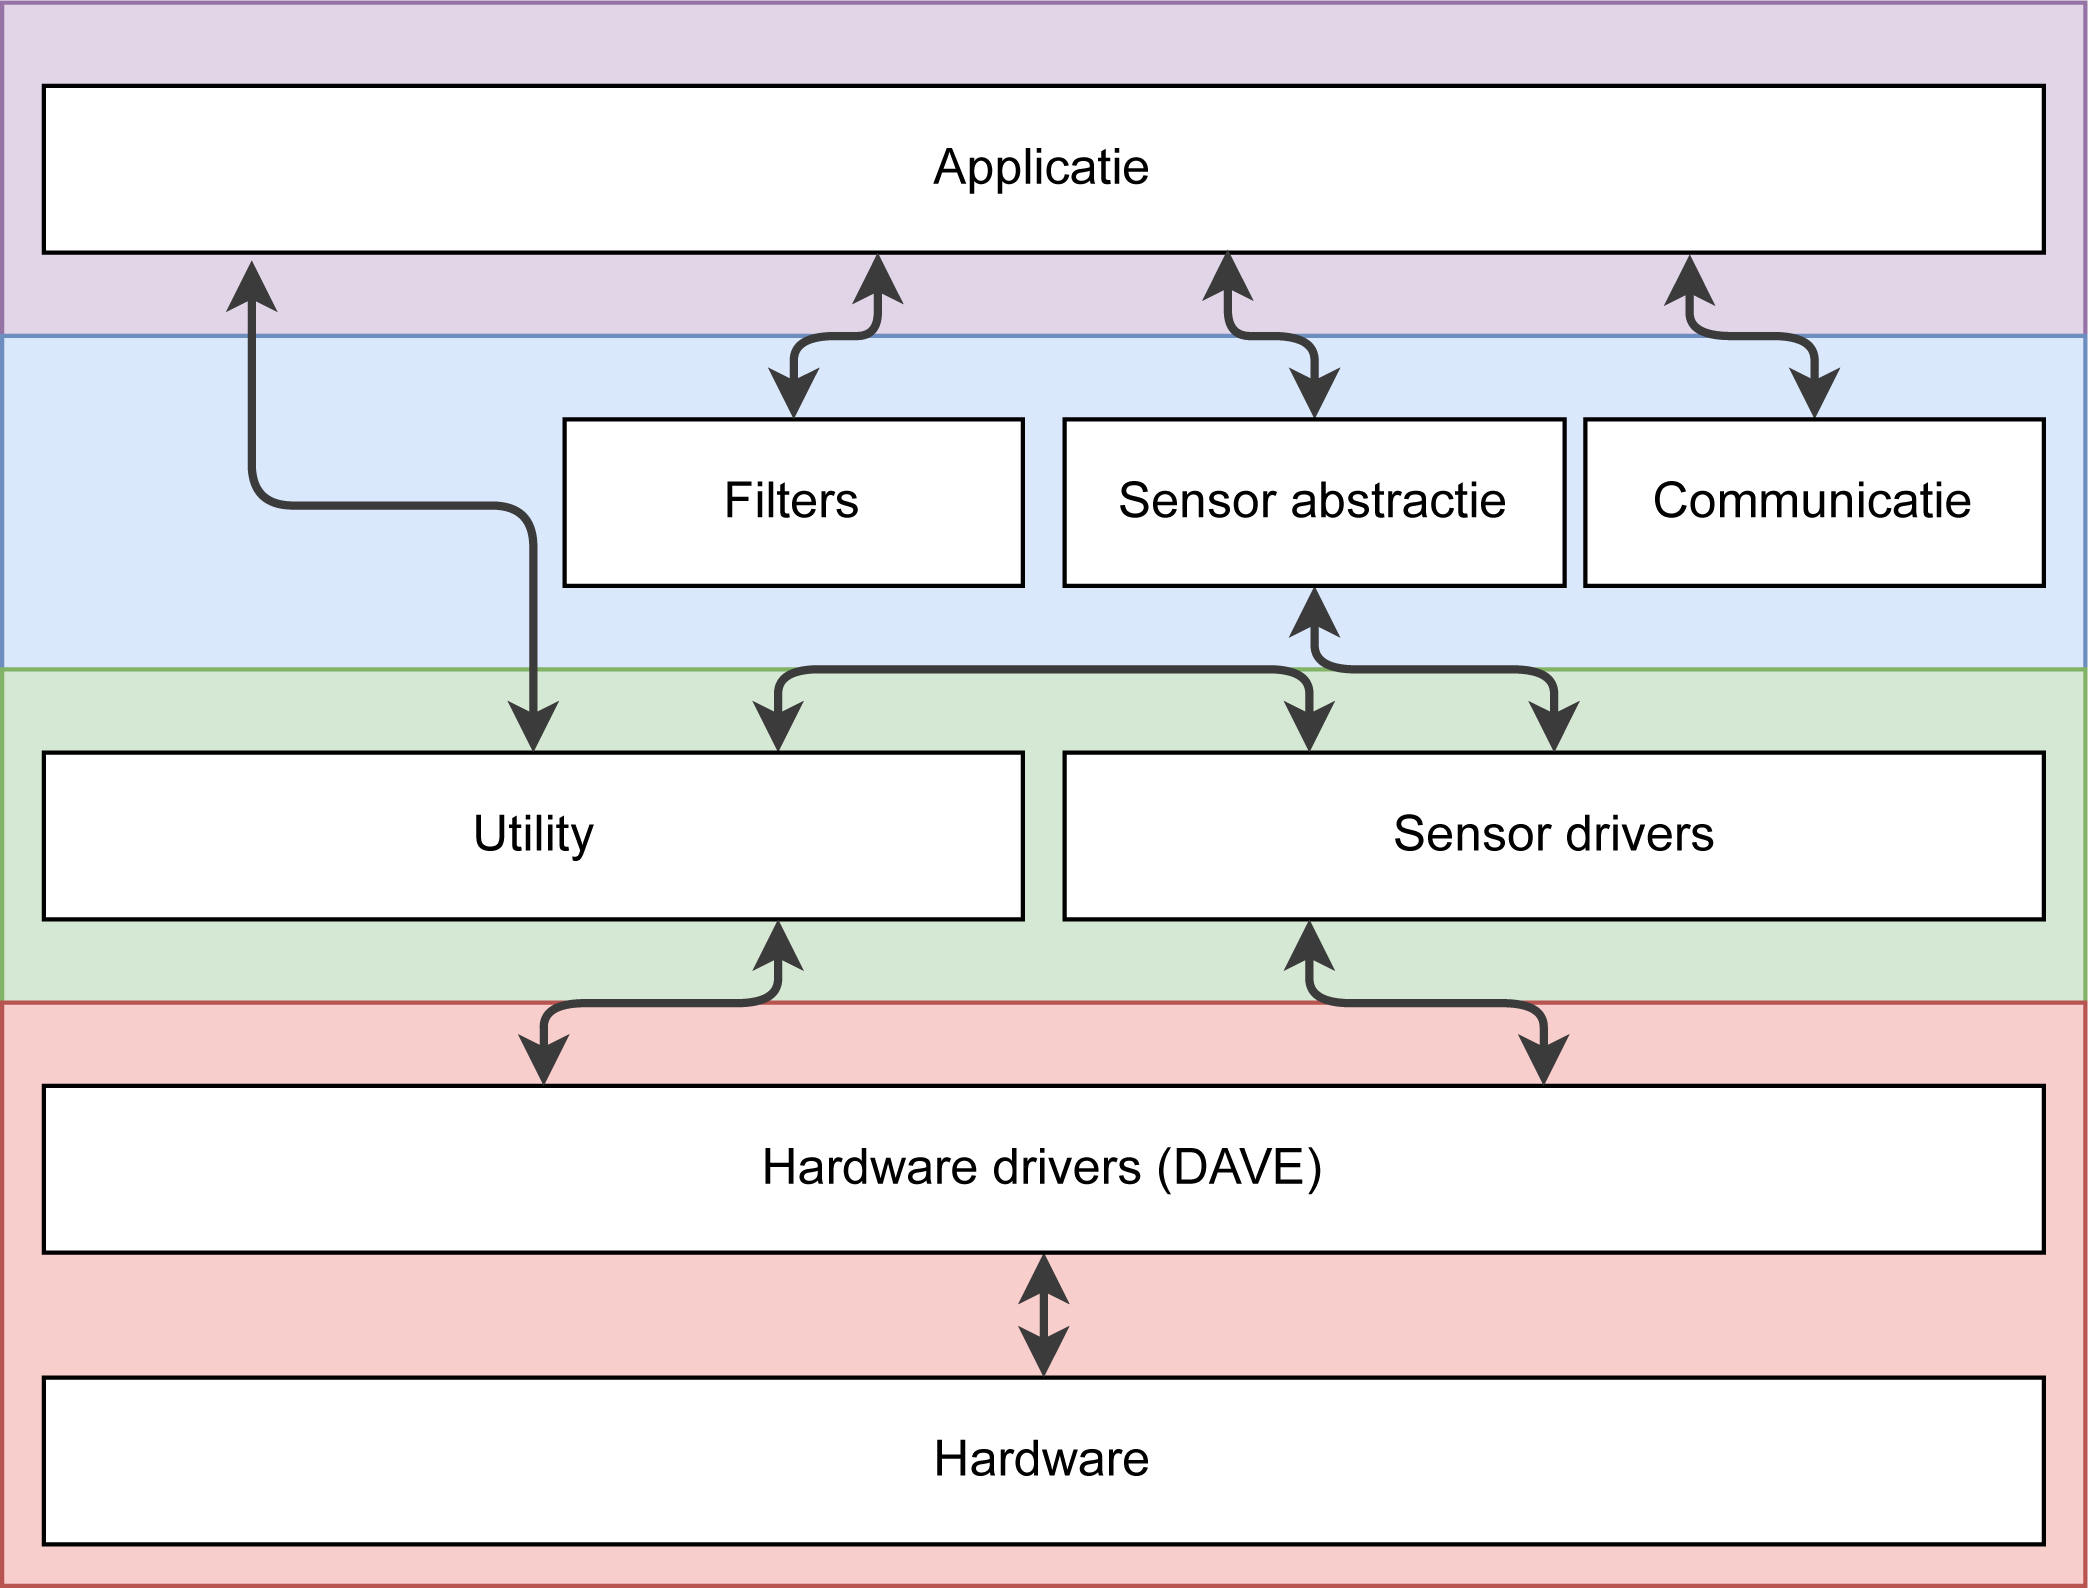
\includegraphics[width=1\linewidth]{ontwerp/applicatie/structuur.jpg}
	\caption{De applicatie ontwerp in lagen}
\end{figure}



\subsection{Applicatie states}
De applicatie is zo ontworpen dat er gebruikt gemaakt wordt van verschillende states en taken die om de bepaalde tijd uitgevoerd moet worden. Deze states zijn tijdvariant maar sommige states zijn juist weer tijdsinvariant. Een tijdvariant taak  betekent dat om zoveel milliseconden er een taak uitgevoerd zal worden. In het ontworpen systeem wordt er om de 100 ms een akkoord gegeven aan de applicatie om sensor data op te halen en uiteindelijk opgestuurd te worden. Een belangrijk onderdeel van de applicatie is de communicatie, het is ontworpen dat er om de seconden sensor data opgestuurd wordt via UDP. Een tijdsinvariant taken zijn taken die niet op tijd gebaseerd zijn. De GNSS Sensor stuurt bijvoorbeeld continue data op. Dit betekent dat er verschillende taken zijn die uiteindelijke allemaal samengevoegd moet worden, hieronder is te zien \ref{fig:appstates} hoe de applicatie dit oplost. \newline

\begin{figure}[h!]
	\centering
	\label{fig:appstates}

	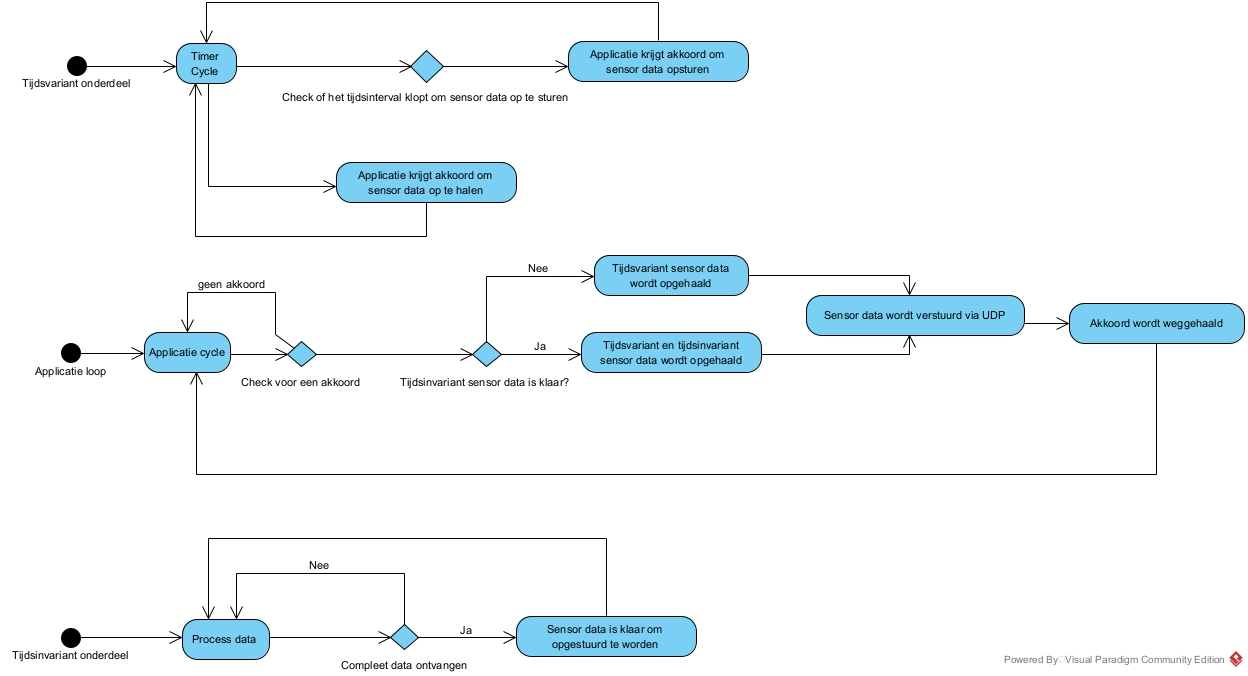
\includegraphics[width=0.73\linewidth]{ontwerp/applicatie/ApplicationStates.jpg}
	\caption{Applicatie states van de applicatie}
\end{figure}

\noindent In het figuur \ref{fig:appstates} zijn er een aantal start nodes, ten eerste is de tijdsvariant onderdeel. Dit wordt per 100 milliseconden uitgevoerd, er wordt hier alleen gecheckt of de applicatie sensor data mag ophalen of verzenden. De applicatie krijgt om de 100 milliseconden dus de tijd om een signaal te geven aan de applicatie loop dat het tijdvariant sensor data opgehaald mag worden. Er mag pas data opgestuurd worden als een bepaald tijdsinterval gehaald wordt, het ontworpen systeem zal dit om 1 seconden doen. Dit betekent voor 10 timer cycles mag er een keer data opgestuurd worden. Bij de 10de cycle wordt er weer signaal gegeven aan de applicatie loop dat er data opgestuurd mag worden. \newline

\noindent Naast het tijdsvariant onderdeel is er ook een tijdsinvariant onderdeel. Dit wordt gebruikt voor sensoren die bijvoorbeeld continue data opsturen naar de Satellite. Dit onderdeel slaat alleen data en als het een compleet sensor packet heeft dan geeft het een signaal aan de applicatie dat er een sensor packet verstuurd kan worden. \newline

\noindent Het laatste onderdeel is de applicatie loop, hier wordt de tijdvariant sensor data opgehaald en uiteindelijk opgestuurd. Er wordt als eerst gecheckt of er een akkoord is om sensor data op te halen of te versturen, als die er is dan haalt hij de tijdsvariant data op, en vervolgens wordt er gekeken of er een tijdsinvariant sensor packet klaar staat. Als dat is wordt het tijdsinvariant packet opgehaald en samengevoegd, en opgestuurd via UDP. Mocht dit niet zijn dan wordt alleen het tijdsvariant sensor data opgehaald en gelijk opgestuurd. \newline

\section{Preprocessor} \label{sec:preprocessor}
De preprocessor is een handig onderdeel van de C taal en een belangrijk onderdeel van het project. De preprocessor is een stap wat voor het compileren gebeurt wordt. Met bepaalde definities in de code kunnen sommige onderdelen niet gecompileerd worden of juist wel. Dit betekent dat makkelijk onderdelen uitgezet kan worden, bijvoorbeeld een specifieke sensor hoeft niet gebruikt te worden, normale wijze zou je dan een if statement maken. Dit betekent alleen wel dat alle code mee gecompileerd zou worden. Met de preprocessor voeg je weer een if statement toe maar dan hoeft de code niet aangepast te worden, er hoeft alleen maar definitie verwijderd worden of toegevoegd worden. Dit betekent dat hele stuk logica niet weggehaald hoeft te worden, de preprocessor bepaald dan of bepaalde onderdelen gecompileerd worden of niet, dit verminderd de compilatie tijd en de uiteindelijk grootte van het programma \autocite{preprocessor}. 

\section{Sensor drivers en abstractie}
Voor de sensoren zijn er twee lagen ontwikkeld, namelijk de drivers en de abstractie. Dit is opgesplitst om de software zo generiek mogelijk te maken. Er wordt dan ook hier naar de volgende deelvraag bekeken \textbf{Op welke manier moet de software ontworpen worden zodat het makkelijk uitbreidbaar is voor nieuwe sensoren?} \newline 

\noindent De drivers en abstractie zijn opgesplitst zodat de applicatie structuur niet aangepast hoeft te worden, er zal dan alleen een nieuwe driver geschreven moeten worden en de abstractie aangepast moeten worden. De driver communiceert met de sensor, en de abstractie is de tussenpersoon tussen applicatie logica en driver. De applicatie zal dan niet veranderen. Om een voorbeeld te geven, de applicatie heeft een poll timer. Deze timer haalt om de 100 milliseconden data op van de inertial measurement unit. Mocht Sensor Maritime een nieuwe inertial measurement unit ondersteunen, normaal zou dan de applicatie logica ook aangepast moeten worden met bepaalde sensor drivers functies. De sensor abstractie vervangt dit het idee is dan ook dat in toekomst de applicatie laag code zo min mogelijk aangepast moet worden. De sensor abstractie moet dan juist aangepast worden en de applicatie laag roept dan de sensor abstractie code op. Hieronder is een overzicht \ref{fig:SensorAbstractie} te zien hoe het dan zou werken. De sensor keuze wordt makkelijk gedaan met de preprocessor (zie hoofdstuk \ref{sec:preprocessor}), hiermee worden sommige sensoren niet gecompileerd of juist wel.
\begin{figure}[h!]
	\centering
	\label{fig:SensorAbstractie}

	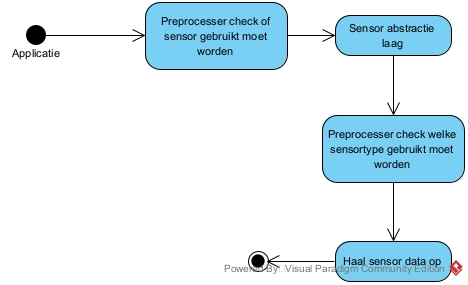
\includegraphics[width=0.46\linewidth]{ontwerp/applicatie/SensorAbstractie.jpg}
	\caption{Sensor abstractie activity diagram}
\end{figure}
	
	
\newpage
\section{Communicatie}
De Satellite heeft verschillende communicatiemiddelen, onder anderen ethernet en CAN Bus. Er zal gefocust worden op communicatie via CAN Bus aangezien dit het meest complex opgebouwd is.  De communicatie via CAN moet voldoen aan de volgende deelvraag: \textbf{Hoe kan er een robuuste communicatie gecreëerd worden tussen het hoofdsysteem en Satellite?} Er moet gekeken worden hoe dit stabiel en robuust gedaan kan worden.\newline


\noindent CAN is een groot onderdeel van de Sensor Maritime infrastructuur. De CAN-communicatie wordt gebruik om te kunnen communiceren met het hoofdsysteem. Hiervoor wordt een master en slave configuratie gebruikt. Het hoofdsysteem is de master en de Satellite en andere eindsystemen zullen dan de slave zijn. De master bepaalt hoe een slave apparaat zich gaat gedragen. CAN staat voor controlled area network, en maakt gebruik van een broadcast systeem. Dit betekent dat alle eindsystemen alle berichten ontvangen, De master kan niet specifiek naar een slave data sturen \autocite{can}. \newline

\noindent Sensor Maritime heeft een eigen protocol ontwikkeld wat gebouwd is op het CAN Bus protocol. Dit zal deels aangepast moeten worden om de Satellite sensoren te kunnen ondersteunen. Het huidige protocol is in afbeelding \ref{fig:canprotocol} te zien. Het protocol is opgebouwd uit velden wat uit 1 of 2 bytes bestaat. In tabel \ref{tab:cansensorprotocol} wordt beschreven wat de taak is van elk veld.
\begin{figure}[h!]
	\centering
	\label{fig:canprotocol}
	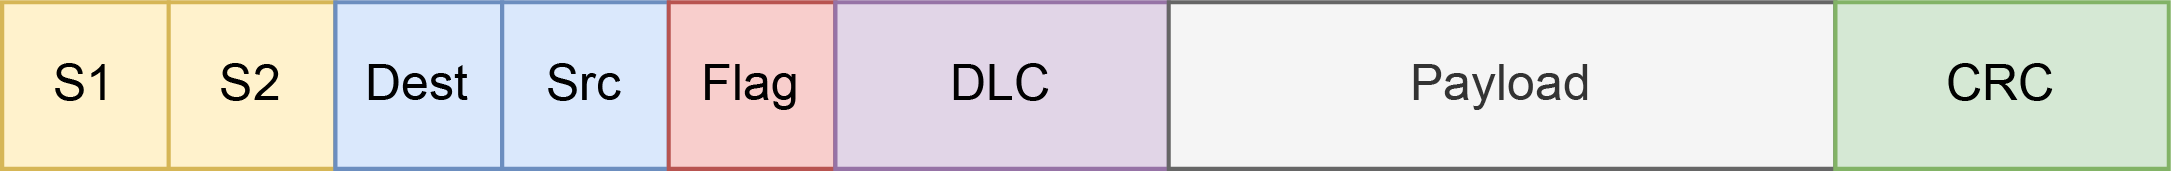
\includegraphics[width=0.75\linewidth]{voorstudie/communicatie/can.png}
	\caption{Sensor Maritime CAN protocol}
\end{figure}

\begin{table}[h!]
	\caption{Sensor Maritime CAN protocol opbouw}
	\label{tab:cansensorprotocol}
	\begin{tabular}{p{1.5cm}p{11.5cm}p{3cm}}
	\toprule
	\textbf{Blok} & \textbf{Beschrijving} & \textbf{Waarde}\\ \midrule
	S1		& De eerste start byte, dit geeft de start aan van het CAN bericht en wordt gebruikt voor herkenning, dit is een vaste waarde.	& 0x40 \\
	S2		& De tweede start byte, dit geeft de start aan van het CAN bericht en wordt gebruikt voor herkenning, dit is een vaste waarde. & 0x02 \\
	Dest	& Deze byte beschrijft voor wie het bericht bedoeld is.		& Verschillend per apparaat. \\
	Src		& Deze byte beschrijft van welke apparaat het bericht komt	& Verschillend per apparaat.\\ 
	Flag	& Dit geeft aan wat voor type bericht het is.             & 0 voor commando \\ 
			& & 1 voor request \\ 
	DLC		& DLC is een afkorting voor Data Length Code.             & \\ 
	Payload	& De data, dit verschillende aan de hand van de flag. & Verschillend per bericht\\
	CRC		& CRC staat voor Cyclic Redundancy Check, dit beschrijft hoe groot het bericht is wat verstuurd wordt. Hiermee kan de ontvanger valideren of het juiste is ontvangen. & Verschillend per bericht\\ \bottomrule
	\end{tabular}
\end{table}

\newpage
\subsection{Probleemstelling}
De huidige CAN BUS protocol ondersteunt de Satellite nog niet. De Satellite is een universeel systeem, waarmee verschillende sensoren verbonden zijn. Het huidige protocol is zo opgebouwd dat er maar één payload opgestuurd kan worden. Dit betekent dat als de Satellite twee sensoren op wil sturen het in de payload gestopt moet worden. Hiervoor moet een vaste structuur bepaald worden zodat de ontvanger weet wat er ontvangen wordt. Om dit probleem op te lossen zal er een aanpassing gemaakt moeten worden aan de bestaande CAN-protocol payload van Sensor Maritime. Hiervoor zijn verschillende oplossingen bedacht die hieronder worden beschreven. Uiteindelijk wordt toegelicht welke oplossing gekozen wordt en waarom. Voor alle payload structuren die beschreven worden zal er gebruik gemaakt worden van hetzelfde voorbeeld. Voor de voorbeelden worden er twee sensoren gebruikt die de Satellite zal ondersteunen. Deze twee sensoren zijn de inductie sensor en de altimeter sensor. De sensoren zullen gerepresenteerd worden als een getallen-lijst die begint bij 0. In het huidige systeem zijn er maar twee sensoren. Dit kan in de toekomst uitgebreid worden. Tabel \ref{tab:SensorRep} geeft een overzicht van de huidige sensoren en hun identificatie.

\begin{table}[h!]
	\centering
	\caption{Sensor identificatie representatie}
	\label{tab:SensorRep}
	\begin{tabular}{p{4cm}p{6cm}}
	\toprule
	Identificatie & Sensor        \\ \midrule
	0      & Inductor  \\
	1      & Altimeter \\ \bottomrule
	\end{tabular}%
\end{table}

\subsection{Structuur 1}
De eerste structuur is ontworpen om zo simpel mogelijk te zijn. Het idee bij dit ontwerp is dat er een identificatie is wat de sensor aangeeft en vervolgens gelijk de waarde van de sensor. Daarnaast voegt dit ook maar 1 byte toe aan de payload per sensor. Dit betekent dat het totale packet maar een aantal bytes groter zal zijn. De afbeelding \ref{fig:Structure1} geeft de opbouw en een voorbeeld weer, hierbij zijn twee sensoren te zien met de identificatie en de waarden van de sensor.
\begin{figure}[h!]
	\centering
	\label{fig:Structure1}


	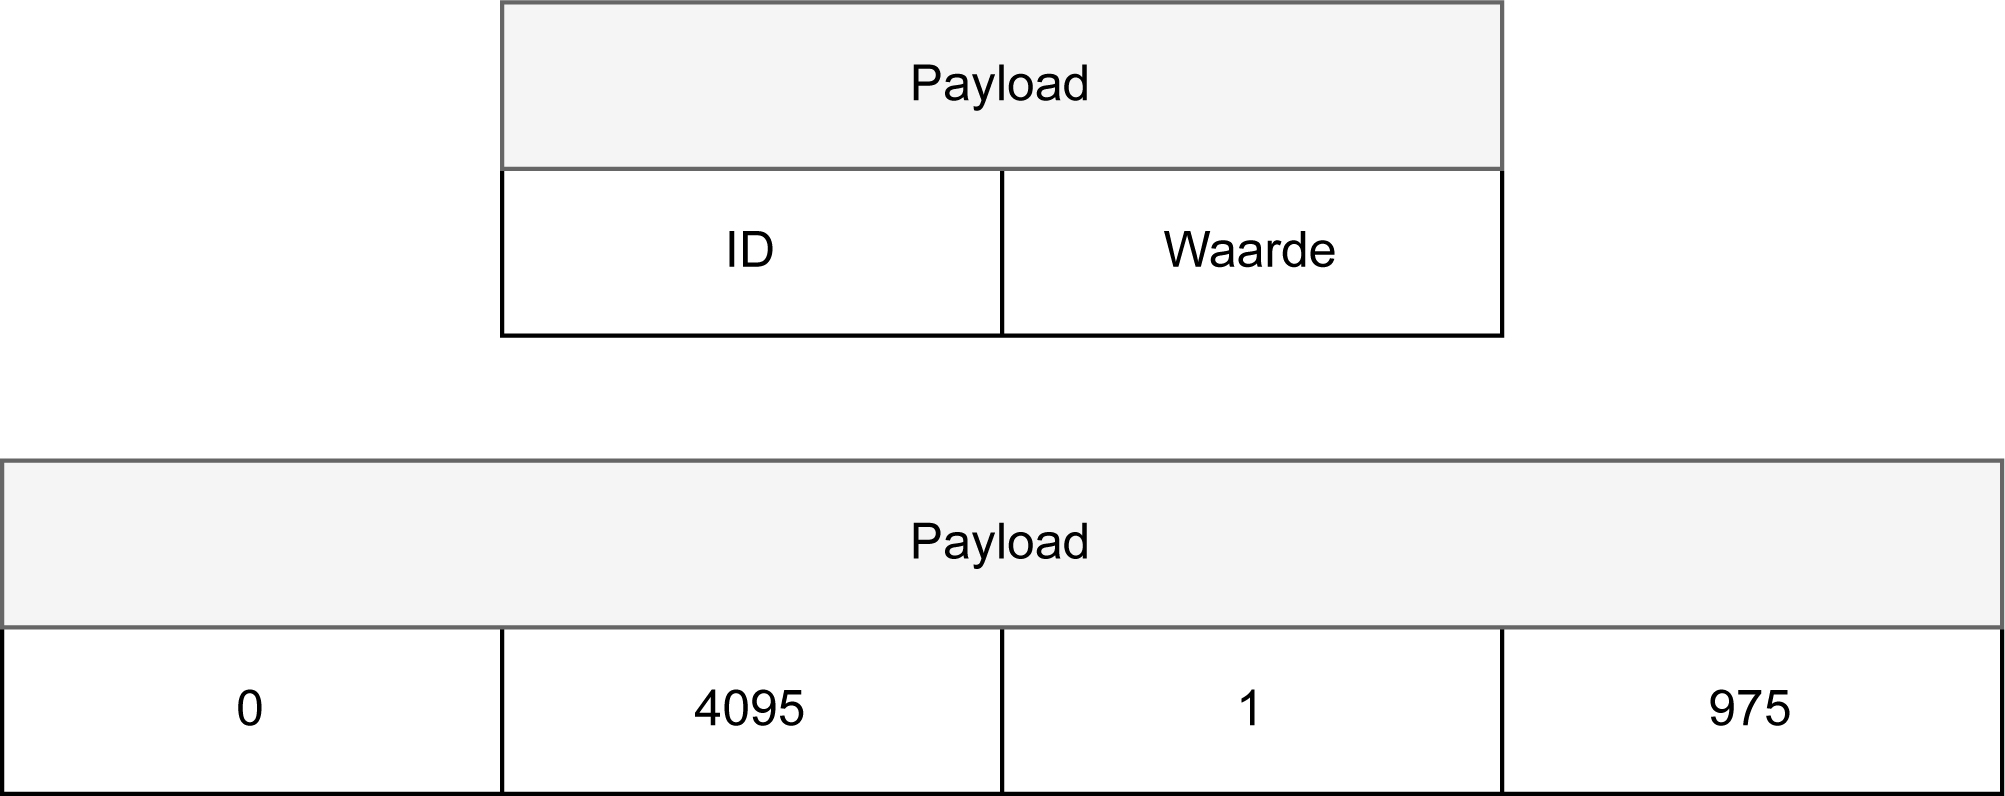
\includegraphics[width=0.75\linewidth]{voorstudie/communicatie/PayloadStructure1-01.jpg}
	\caption{Opbouw en voorbeeld van de payload structuur 1}
\end{figure}

\newpage
\subsection{Structuur 2}
Structuur 2 is opgezet om zoveel mogelijk te ondersteunen. Ten eerste ondersteunt dit meerdere datatypes, bijvoorbeeld 8, 16, 32 bit nummers maar ook 32 bit en 64 bit decimalen. Ten tweede geeft deze structuur duidelijk aan wat de grootte is van een packet. Packet grootte, geeft aan de hele sensor packet grootte in bytes. De identificatie geeft aan wat voor sensor het is. Dan komen er drie kolommen voor de waarde. Eerste wordt de waarde grootte in bytes gegeven, dan de waardetype en uiteindelijk de waarde zelf. In de volgende afbeelding \ref{fig:Structure2} is een overzicht te zien.
\begin{figure}[h!]
	\centering
	\label{fig:Structure2}

	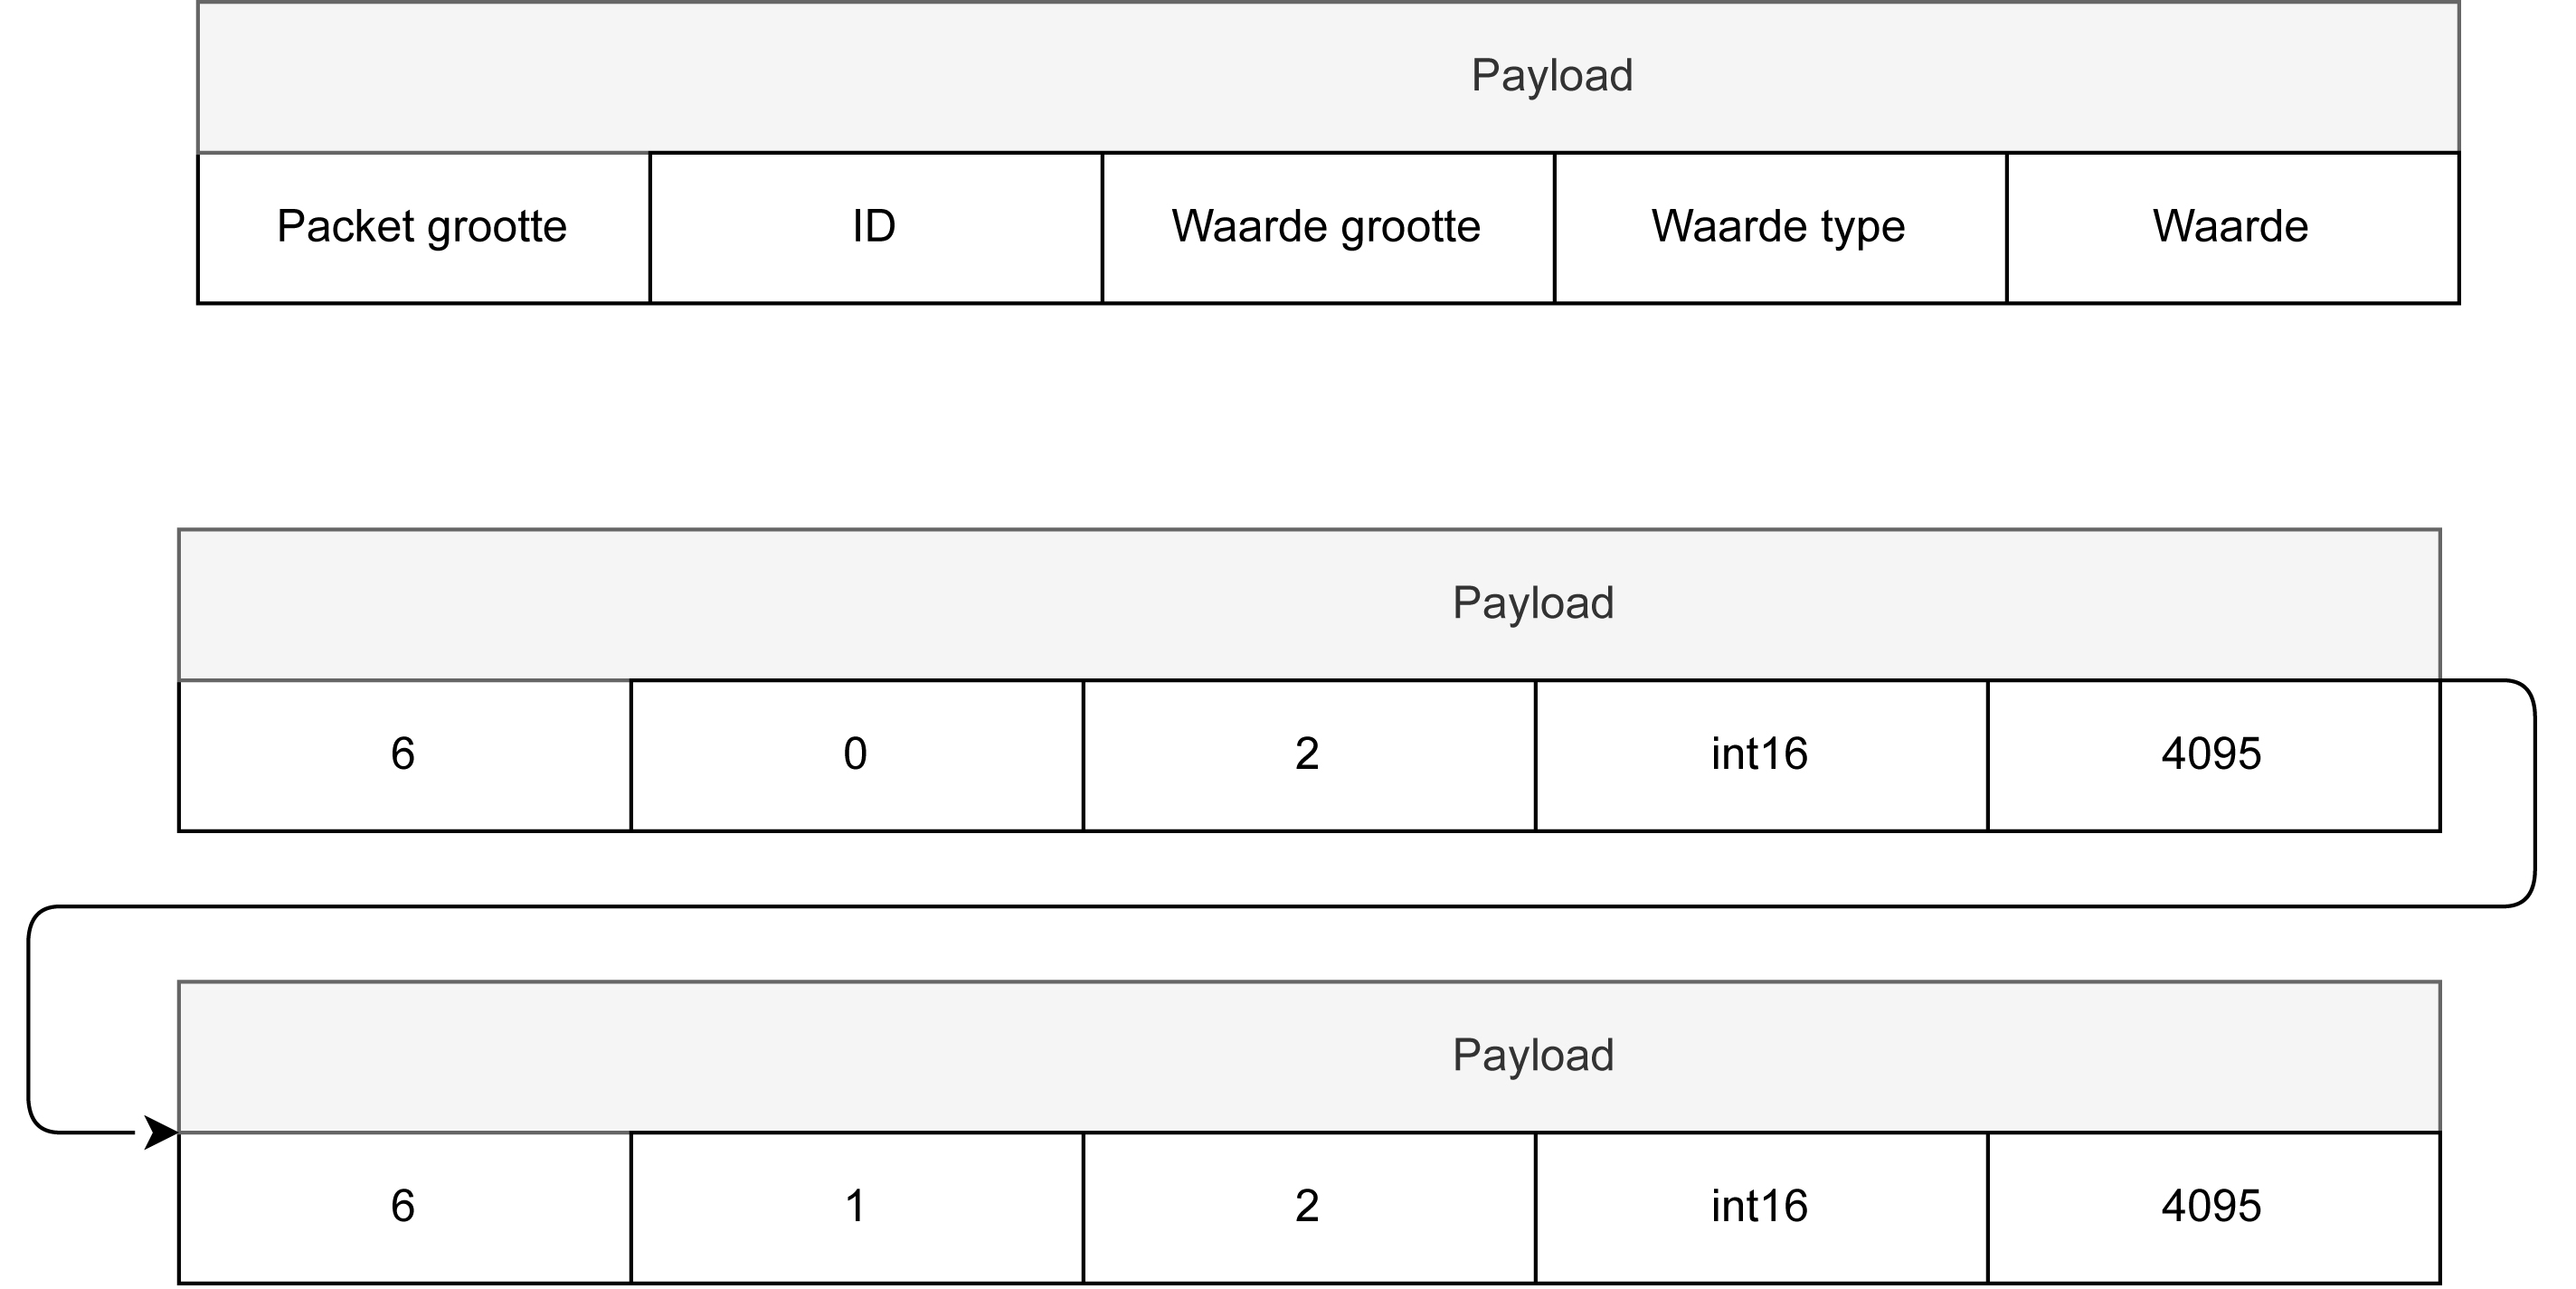
\includegraphics[width=0.75\linewidth]{voorstudie/communicatie/PayloadStructure2-01.jpg}
	\caption{Opbouw en voorbeeld van de payload structuur 2}
\end{figure}

\subsection{Structuur 3}
Dit is de laatste structuur die ontworpen is. Het is een combinatie van structuur 1 en structuur 2. Deze structuur heeft drie onderdelen voor een sensor. Als eerste zal de sensor identificatie meegegeven worden. Daarna komt de waarde grootte in bytes, en uiteindelijk wordt de waarde zelf gegeven. In afbeelding \ref{fig:Structure3} wordt de structuur en een voorbeeld weergeven.
\begin{figure}[h!]
	\label{fig:Structure3}

	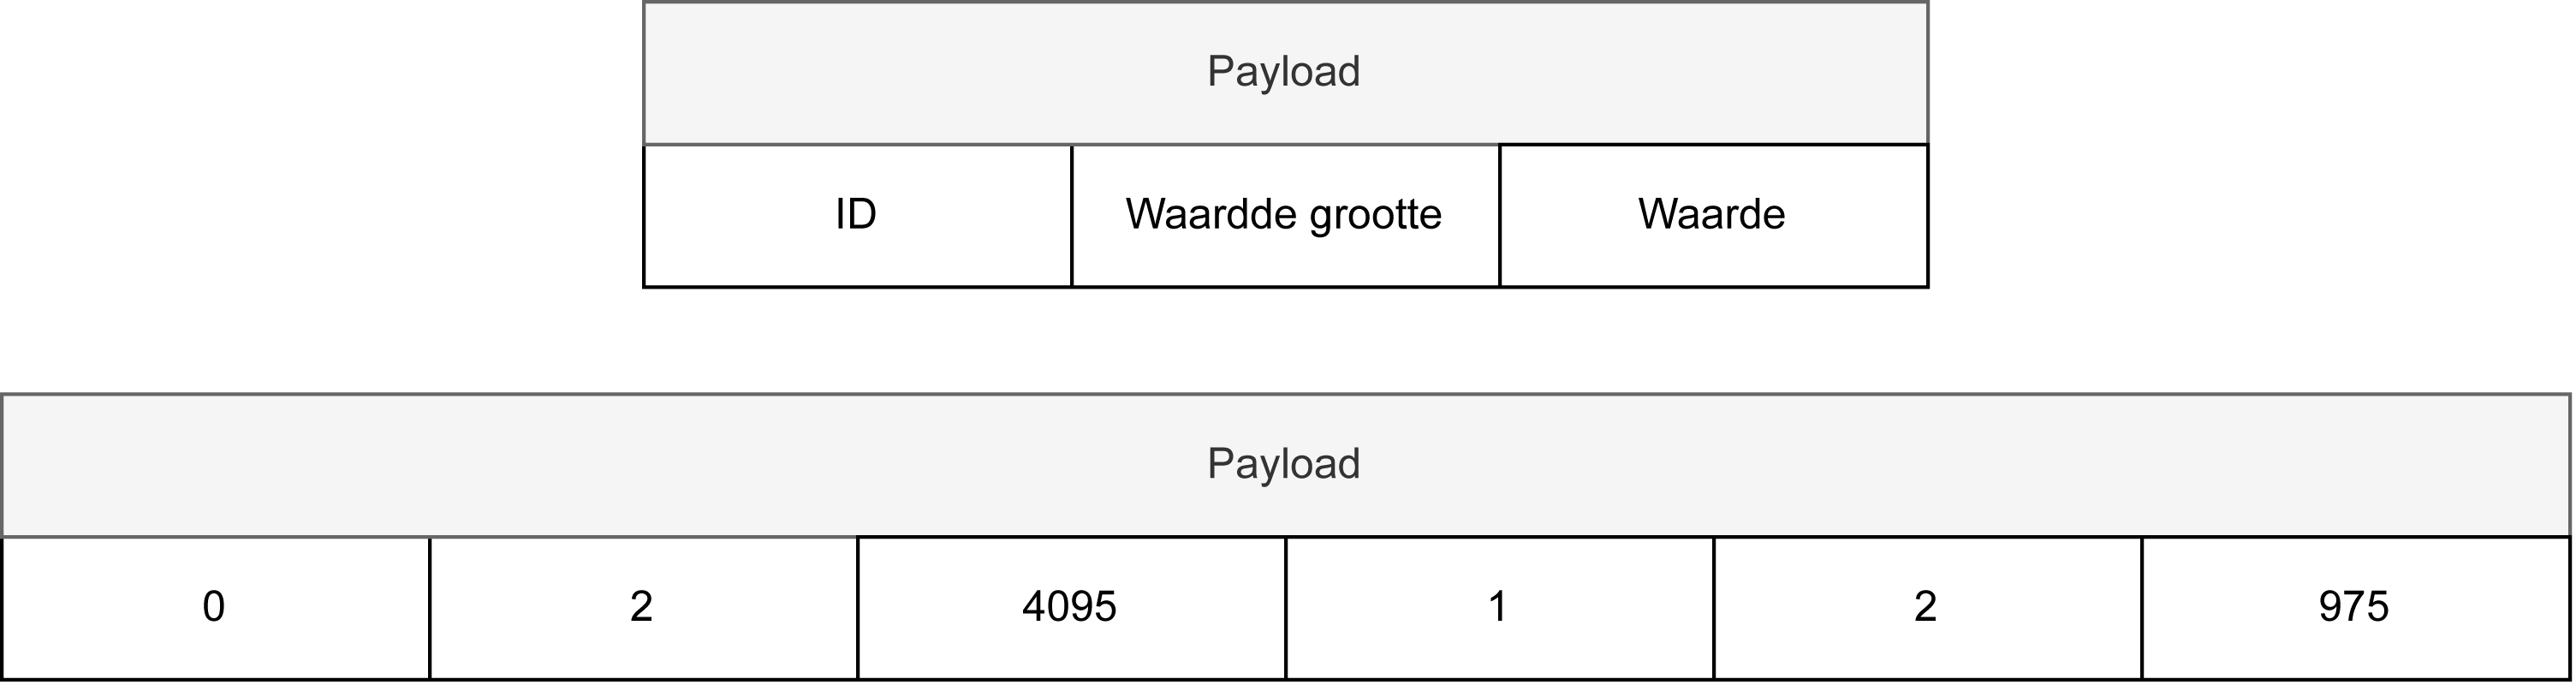
\includegraphics[width=\linewidth]{voorstudie/communicatie/PayloadStructure3-01.jpg}
	\caption{Opbouw en voorbeeld van de payload structuur 3}
\end{figure}

\newpage
\subsection{Communicatie flow}
Hieronder is in in figuur \ref{fig:comflow} te zien hoe de communicatie via CAN-bus gedaan wordt als er een bericht ontvangen wordt van het eindsysteem. Om een connectie te creëren zijn een aantal stappen nodig om dit goed af te handelen. Het hoofdsysteem kan verschillende type berichten sturen, in het vorige hoofdstuk is er vooral gefocust op de sensor payload structuur. Maar voor elk type bericht zal het apart afgehandeld worden. Er wordt dus eerst gecheckt wat voor type bericht het is, en daarvan splits het op in twee sectoren. De linker sector is een simpele structuur waarbij alleen wat data opgehaald of een karakter meegegeven moet worden. Bij de rechter sector wordt de payload structuur opgezet als eerste voor elke sensor dat de Satellite heeft. Dan wordt de payload berekend in bytes. Met de grootte in bytes kan het packet gemaakt worden. Vervolgens wordt het opgestuurd, dit zal een status code teruggeven. Als de communicatie al bezig is met iets versturen zal hierop gewacht moeten worden. Bij andere errors, failures zal een rood lichtje branden als status.
\begin{figure}[h!]
	\centering
	\label{fig:comflow}

	\includegraphics[width=0.7\linewidth]{ontwerp/communicatie/DataFlow.jpg}
	\caption{Activity diagram van de communicatie}
\end{figure}

\newpage
\subsection{Conclusie}
In dit subhoofdstuk is gekeken naar een manier om de huidige CAN Bus protocol zo aan te passen zodat het beter aansluit op de Satellite. De Satellite heeft verschillende sensoren die allemaal uiteindelijk in een payload moeten komen. Omdat het hoofdsysteem niet weet wat voor sensoren de Satellite op enig moment heeft, betekent het dat dit problemen kan veroorzaken. De nieuwe structuur voor de payload moet simpel te implementeren zijn, maar de payload moet ook niet veel groter worden. De eerste structuur is het simpelste maar is lastiger om te implementeren. Het grootste probleem is dat de buffer niet weet waar de volgende sensor begint. De waarde van sensor kan bijvoorbeeld 2 bytes zijn of 8 bytes. Het voordeel van structuur 1 is dat het een kleine structuur is waardoor de totale hoeveelheid data die opgestuurd wordt niet veel groter wordt. Structuur 2 is het tegenovergestelde van structuur 1, structuur 2 is makkelijk te implementeren omdat precies gezien kan worden wat verwacht kan worden per byte. Het probleem van structuur 2 is dat het veel groter is in bytes. Uiteindelijk is er nog structuur 3 en die zit tussen structuur 1 en 2, in vergelijking met hoe simpel het is om te implementeren en packet grootte. Een samenvatting van de structuren is te vinden in tabel \ref{tab:samenvattingstructuur}. \newline

\begin{table}[h!]
	\centering
	\caption{Samenvatting van CAN Payload structuren}
	\label{tab:samenvattingstructuur}
	\begin{tabular}{lll}
	\toprule
		Structuur nummer & Implementatie moeilijkheid & Packet grootte             \\ \midrule
		1                & Lastig                     & Klein (2 tot 9 bytes)      \\
		2                & Simpel                     & Groot (5 tot 12 bytes)     \\
		3                & Simpel                     & Gemiddeld (3 tot 10 bytes) \\ \bottomrule
	\end{tabular}%
\end{table}

\noindent In dit subhoofdstuk is er gekeken naar de volgende deelvraag \textbf{Hoe kan er een robuuste communicatie gecreëerd worden tussen het hoofdsysteem en Satellite?} Er is gekeken naar de moeilijkheid van de implementatie en de grootte van de payload. Deze twee onderdelen spelen een belangrijk onderdeel bij een robuuste communicatie. Daarom is er gekozen voor structuur 3, dit is een vrij simpele implementatie, en vergroot de payload maar weinig. Met deze payload-structuur weet het hoofdsysteem precies wat er gaat komen en hoeveel sensoren aan de Satellite verbonden zijn.
\newpage

\newpage
\section{Validatie}
Elke nieuwe hardware wat aan Satellite wordt geleverd zal door Sensor Maritime moeten gevalideerd moeten worden. Er zal als eerst beschreven worden welke porten er getest worden. De volgende type porten worden besproken. Ten eerste zal er gekeken worden naar DIP schakelaars, digitale output, analoge input, relay en uiteindelijk seriele communicatie. \newline

\noindent De Satellite heeft verschilllende porten porten zijn die gebruikt kan worden. Elke type port wordt beschreven in de volgende hoofdstukken. In deze hoofdstukken wordt beschreven wat de port moet doen en hoe dit getest gaat worden en uiteindelijk wat het verwachte resultaat is.

\subsection{DIP switch}
Een DIP switch bestaat uit een aantal schakelaars die je kan of uit kan zitten \autocite{DIP}. Op de Satellite is er een DIP switch aan bord, die acht schakelaar is heeft. Zeven van de acht worden op het moment gebruikt. Het volgende tabel \ref{tab:hw_val_dip} geeft aan wat de acties zijn als je de schakelaar aan of uit zet. De eerste drie van de schakelaars worden gebruikt als configuratie voor andere porten die worden beschreven in hoofdstuk \ref{Analog Input Signaal}. De laatste vier schakelaars zetten een specifiek pin van de microcontroller hoog of laag.
\begin{table}[h!]
	\caption{DIP switch porten die gevalideerd moeten worden}
	\begin{tabular}{llllp{10cm}}
	\toprule
	\textbf{Naam} & \textbf{GPIO} & \textbf{Pin} & \textbf{IO} & \textbf{Beschrijving}	\\ \toprule
	PU1		& -			& - 	& -    		& Verandert de analog input 1 voltage tussen 0 en 24V	\\
	-		& -			& - 	& -    		& Wordt niet gebruikt.								\\
	PU2		& -			& - 	& -    		& Verandert de analog input 2 voltage tussen 0 en 24V	\\
	PU3		& -			& - 	& -    		& Verandert de analog input 3 voltage tussen 0 en 24V	\\
	ADD0 	& 3			& 10	& Input		& Zet de pin hoog of laag, aan de hand van of het aan staat of niet.		\\
	ADD1 	& 3			& 11	& Input		& Zet de pin hoog of laag, aan de hand van of het aan staat of niet.		\\
	ADD2 	& 3			& 12	& Input		& Zet de pin hoog of laag, aan de hand van of het aan staat of niet.		\\
	ADD3 	& 3			& 0 	& Input		& Zet de pin hoog of laag, aan de hand van of het aan staat of niet.		\\ \bottomrule
	\end{tabular}
	\label{tab:hw_val_dip}
\end{table}

\subsection{Digital output signaal}
De digitale output signaal kan alleen hoog of uit gezet worden, dit betekent dat het geen input modus heeft. De Satellite heeft vier digitale output porten die op 24V of 0V gezet kan worden. Het volgende tabel geeft een overzicht \ref{tab:hw_val_dio}.
\begin{table}[h!]
	\caption{Digital output signalen die gevalideerd moeten worden}
	\begin{tabular}{llllp{10cm}}
	\toprule
	\textbf{Naam} & \textbf{GPIO} & \textbf{Pin} & \textbf{IO} & \textbf{Beschrijving}				 	\\ \toprule
	D1			& 1			& 6    	& Output	& Digital output signaal, op deze pin komt 24V of 0V. \\
	D2			& 1			& 7    	& Output	& Digital output signaal, op deze pin komt 24V of 0V. \\
	D3			& 3			& 3    	& Output	& Digital output signaal, op deze pin komt 24V of 0V. \\
	D4			& 3			& 2   	& Output	& Digital output signaal, op deze pin komt 24V of 0V. \\ \bottomrule
	\end{tabular}
	\label{tab:hw_val_dio}
\end{table}

\subsection{Analog input signaal} \label{Analog Input Signaal}
De analog signalen kan alleen uitgelezen worden, dit betekent dat het alleen een input modus heeft. De Satellite heeft drie analoge input porten aan bord. In het volgende tabel wordt een overzicht gegeven \ref{tab:hw_val_ai}.
\begin{table}[h!]
	\caption{Analog input signalen die gevalideerd moeten worden}
	\begin{tabular}{llllp{9cm}}
	\toprule
	\textbf{IO} & \textbf{GPIO} & \textbf{Pin} & \textbf{Input/Output} & \textbf{Beschrijving}			\\ \toprule
	AI1			& 14		& 2    	& Input		& Analoge input signaal van 0 tot 24 volt.					\\
	AI2			& 14		& 3    	& Input		& Analoge input signaal van 0 tot 24 volt.					\\
	AI3			& 14		& 12   	& Input		& Analoge input signaal van 0 tot 24 volt.					\\  \bottomrule
	\end{tabular}
	\label{tab:hw_val_ai}
\end{table}

\subsection{Relay}
Er is een relay verbonden aan de microcontroller. Een relay is een mechanisch apparaat dat een elektrische connectie maakt tussen twee of meer punten op reactie van de microcontroller. Als er 3,3 volt op de relay gezet wordt zal de relay sluiten en bij 0 volt zal het weer openen gaan. Omdat het mechanisch is moet je dit ook kunnen horen \autocite{relay}. Hieronder is een overzicht van de relay \ref{tab:hw_val_relay}.

\begin{table}[h!]
	\caption{Relay signaal die gevalideerd moeten worden}
	\begin{tabular}{llllp{9cm}}
	\toprule
	\textbf{IO} & \textbf{GPIO} & \textbf{Pin} & \textbf{Input/Output} & \textbf{Beschrijving}			\\ \toprule
	Relay		& 3 & 1   	& Output		& Een mechanische apparaat was dicht of opengaat aan de hand of er 3,3 volt of niet op staat.	\\ \bottomrule
	\end{tabular}
	\label{tab:hw_val_relay}
\end{table}

\subsection{Serieel Communicatie}
De Satellite heeft verschillende porten voor seriele communicatie aanbord. De seriele communicatie middelen zullen gebruikt worden voor communicatie met een eindsysteem of sensoren. Sommige sensoren die Sensor Maritime gebruiken sturen de gegevens via seriele communicatie over. Omdat het zoveel functionaliteiten heeft zal dit grondig getest moeten worden. Satellite heeft verschillende varianten van seriele communicatie, ten eerste zijn er twee UART verbindingen, een RS232 verbinding, en uiteindelijk een RS422 communicatie lijn. \newline

\noindent UART staat voor Universal asynchronous receiver-transmitter. UART stuurt asynchroon data over dit betekent dat er geen klok signaal is die data synchroon maakt. UART wordt universeel genoemd omdat het geconfigureerd om verschillende seriele protocollen te ondersteunen. In plaats van een klok signaal wordt er gebruikt gemaakt van een start bit en een stop bit. Data wordt verstuurd via UART via de gebruiker gespecificeerd frequentie, dit wordt ook wel baudrate genoemd, baudrate wordt gespecificeerd als in bits per seconden (bps) \autocite{UART}. \newline

\noindent RS-232 is anders opgebouwd dan UART. RS-232 is een standaard gedefineerd signaal tussen twee apparaten, waar de signaal naam, doel, spanningniveau en pinnen zijn gedefineerd zijn. Een belangrijk verschil tussen RS-232 en UART is dat de spanningniveau hoger en negatief kan zijn. Het voltage bereik van RS-232 gaat -12 volt tot 12 volt \autocite{RS232}. \newline

\noindent RS-422 is weer een andere vorm van seriele communicatie en heeft kenmerken van RS-232. Het verschil tussen RS-232 en RS-422 is dat het voor de communicatie vier lijnen gebruikt (RX-, RX+, TX+, TX-). Met de vier communicatielijnen kan er full duplex gecommuniceerd worden. Full duplex communicatie betekent dat er twee of meer apparaten in beide richting kan communiceren (ontvangen en verzenden op hetzelfde moment) \autocite{FullDuplex}. RS-232 heeft half-duplex dit houdt in dat via RS-232 alleen handeling gedaan kan worden, bijvoorbeeld eerst ontvangen en dan pas verzenden. \autocite{RS422}.

\noindent In het volgende tabel \ref{tab:hw_val_serieel}wordt een overzicht gegeven van de seriele communicatie die verbonden zijn op de microcontroller. Voor de RS-422 communicatie is alleen twee communicatielijnen aangegeven, omdat dit zo verbonden is op de microcontroller. De Rx+, RX- en TX+, TX- lijnen worden samengevoegd door een chip en dan verbonden naar de microcontroller.
\begin{table}[h!]
	\caption{Seriele communicatie porten die gevalideerd moeten worden}
	\begin{tabular}{llllp{9cm}}
	\toprule
	\textbf{IO} & \textbf{GPIO} & \textbf{Pin} & \textbf{Input/Output} & \textbf{Beschrijving}	\\ \toprule
	UART RX		& 5			& 0    	& Input		& Seriele communicatie ontvangst lijn.			\\
	UART TX		& 5			& 1    	& Output	& Seriele communicatie versturen lijn.			\\
	RS-232 RX	& 3			& 7    	& Input		& Seriele communicatie ontvangst lijn.			\\
	RS-232 TX	& 3			& 8    	& Output	& Seriele communicatie versturen lijn.			\\
	RS-422 RX	& 6			& 3    	& Input		& Seriele communicatie ontvangst lijn.			\\
	RS-422 TX	& 3			& 13   	& Output	& Seriele communicatie versturen lijn.			\\
	UART 2 RX	& 4			& 6    	& Input		& Seriele communicatie ontvangst lijn.			\\
	UART 2 TX	& 4			& 7   	& Output	& Seriele communicatie versturen lijn.			\\ \bottomrule
	\end{tabular}
	\label{tab:hw_val_serieel}
\end{table}

\newpage
\section{Klasse diagram}
Hieronder is een klasse diagram gegeven van de hele applicatie \ref{fig:klassediagram}. In de klasse diagram is goed is te zien dat alle sensoren een abstractie laag hebben, die specifieke gekoppeld is aan een sensor  driver. De hardware abstractie lagen die door DAVE zijn gemaakt zijn worden niet getoond in de klasse diagram aangezien dit een externe library is.
\begin{figure}[h!]
	\centering
	\label{fig:klassediagram}

	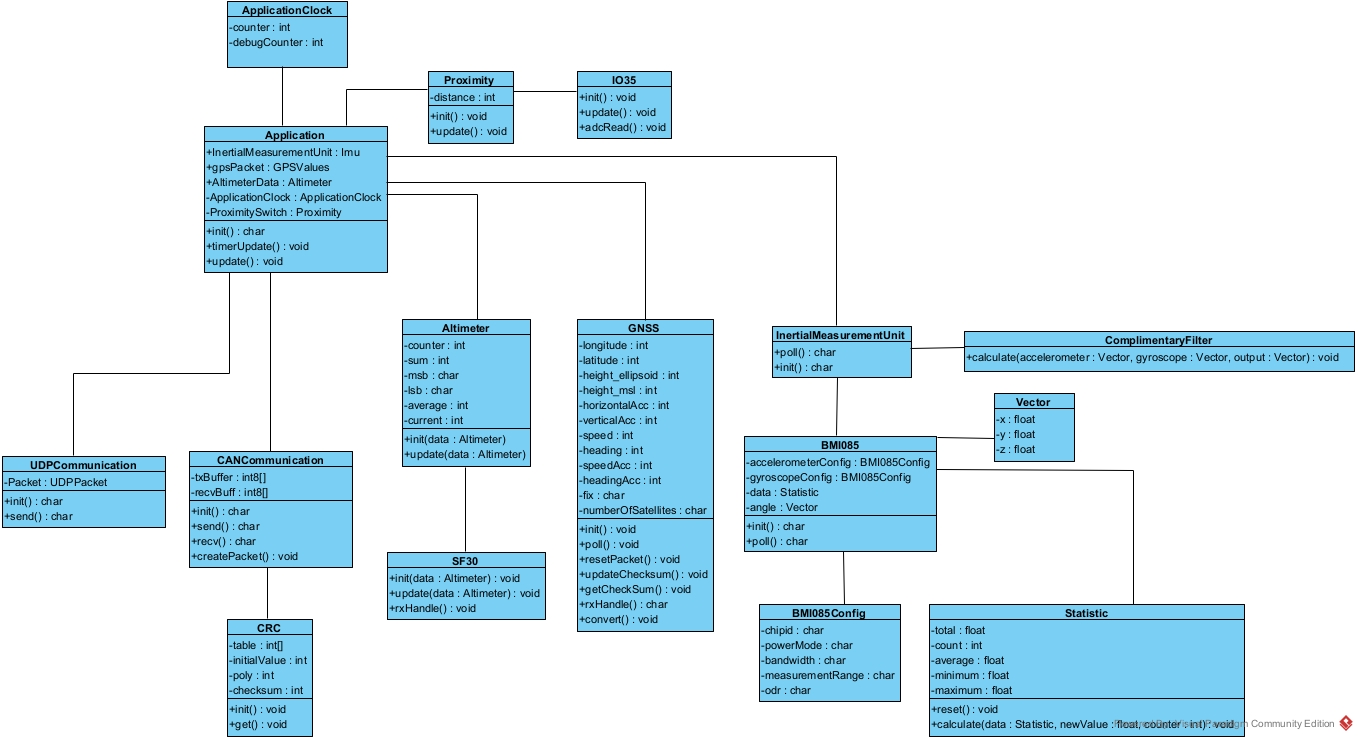
\includegraphics[width=\linewidth]{ontwerp/applicatie/Satellite.jpg}
	\caption{Algemene structuur van de applicatie}
\end{figure}
